\documentclass[12pt]{extarticle}
\usepackage{hyperref}
\usepackage[margin=0.8in]{geometry}
\usepackage{tabularx}
\usepackage{xcolor-material}
\usepackage{cancel}
\usepackage{ulem}
\usepackage{graphicx}

\renewcommand\tabularxcolumn[1]{m{#1}}% for vertical centering text in X column

\begin{document}
\begin{titlepage}
\centering
{\LARGE\bfseries Basi di Dati}

\vspace{1cm}

{\Large Progetto d'esame}

\vspace{0.2cm}
{\large (a.a. 2018-2019)}

\vspace{2cm}

{\large Alexandru MOCANU}

\vspace{0.2cm}

{\small Matr. 813322}


\vspace{2cm}

% {\bfseries Submitted in fulfillment of the degree \ldots}

\vfill

{\itshape Università degli Studi di Torino - Dipartimento di Informatica}
\end{titlepage}

% Other content goes here...
\tableofcontents

\clearpage

\section{Progettazione concettuale}
\subsection{Requisiti Iniziali: SITO RICETTE}
Si vuole realizzare una base di dati per la gestione di una piattaforma in cui gli utenti possano
scoprire e condividere ricette\footnote{La piattaforma descritta è liberamente ispirata al sito Giallo Zafferano 
(\url{www.giallozafferano.it}), a cui è possibile fare riferimento per risolvere eventuali ambiguità nei requisiti}.
Per poter caricare le loro ricette, gli utenti devono registrarsi
fornendo \textbf{email}, \textbf{password} e un \textbf{nome utente} che sarà associato a tutti i loro contributi.
\\\\
Le ricette hanno un titolo, una descrizione, una foto di copertina, alcune informazioni su difficoltà,
tempo di preparazione, ecc. ed una lista di ingredienti. Per ogni ingrediente si
specificano il nome, la quantità ed eventuali annotazioni. Inoltre, ogni ricetta appartiene ad una
categoria che identifica il tipo di portata (es. antipasto, primo piatto, \dots) e, in qualche caso, anche
ad una o più categorie che identificano la dieta associata (es. vegetariana, senza glutine, ...). Oltre
che dagli utenti, le ricette possono essere pubblicate dalla redazione del sito. Le ricette della
redazione possono avere come autore un cuoco famoso.
\\\\
Esplorando la pagina di un cuoco sul sito, i visitatori possono leggerne una
breve bio e accedere a tutte le ricette di cui questi è l’autore (di cui è subito visibile anche il
numero). Gli utenti possono seguire un cuoco per visualizzare le sue ricette in primo piano nella
propria pagina personale.
\\\\
Le persone possono inoltre salvare le ricette tra i propri preferiti e singoli ingredienti in una “lista
della spesa”. I preferiti e le cose da comprare sono visualizzati nella pagina personale degli utenti,
insieme ad un’indicazione del numero di ricette e del numero di commenti pubblicati.
\\\\
I visitatori possono infatti anche commentare le ricette, eventualmente rispondendo ad un
commento già pubblicato da qualcun altro. Anche la redazione può pubblicare dei commenti, ma
solo in risposta ai commenti lasciati dai visitatori. Per ogni commento vengono visualizzati: lo
username e la foto profilo dell’autore (o la dicitura “Redazione”), la data e il testo.
\\\\
Ad ogni ricetta sono associate delle ricette simili. Due ricette si considerano simili se hanno
almeno una categoria in comune e hanno come autore lo stesso cuoco o utente.
\\\\
Quando una persona cancella la propria iscrizione al sito, anche i suoi dati personali sono
cancellati, mentre le ricette che ha condiviso e i suoi commenti vengono mantenuti. Sono invece
cancellati insieme ai dati personali i preferiti, gli ingredienti contenuti nella lista della spesa, la lista
dei cuochi eventualmente seguiti.

\newpage

\subsection{Glossario dei termini}
\vspace{2cm}
    \begin{tabularx}{\textwidth}{X|X|X|X}
    \bfseries Termine      & \bfseries Descrizione  & \bfseries Sinonimo  & \bfseries Collegamenti\\ 
    \hline\hline
    \bfseries Utente       & Persona che si iscrive al sito mediante un nome utente, email e password                                                                                                            & visitatore, persona & ricetta, ingrediuente, commento \\ 
    \hline
    \bfseries Ricetta      & Indicazione relativa agli ingredienti, alle dosi, alla preparazione di una pietanza, di una bevand o di un dolce.                                                              & /                   & utente, ingrediente, commento   \\
    \hline
    \bfseries Ingrediente  & Sostanze che entra a far parte di un prodotto  risulta necessaria all'esecuzione di una ricetta. Di ogni ingrediente viene rappresentato  il nome e la quantità da utilizzare & /                   & utente, ricetta                 \\
    \hline
    \bfseries Commento     & I commenti possono essere scritti da utenti sotto una ricetta, oppure possono essere scritti in risposta ad un altro commento.                                                     & /                   & ricetta, utente                 \\
    \hline
    \bfseries Cuoco famoso & Un cuoco famoso ha un proprio profilo che può esser seguito dagli altri utenti.                                                                                                      & /                   & utente                          \\
    \hline
    \bfseries Redazione    & La Redazione si occupa della pubblicazione delle ricette  risponde ai commenti                                                                                                        & /                   & (ricetta, commento)             \\
    \end{tabularx}

\newpage

\subsection{Requisiti rivisti e strutturati in gruppi di frasi omogenee}

\subsubsection{Requisiti riscritti}
Si vuole realizzare una base di dati per la gestione di una piattaforma in cui gli utenti possano
scoprire e condividere ricette\footnote{La piattaforma descritta è liberamente ispirata al sito Giallo Zafferano 
(\url{www.giallozafferano.it}), a cui è possibile fare riferimento per risolvere eventuali ambiguità nei requisiti}.
Per \textcolor{blue}{gli utenti, che per} poter caricare le loro ricette, \xout{gli utenti} devono registrarsi 
\textcolor{blue}{rappresentiamo nome utente, utilizzato per l'identificazione univoca, email e password}.
\\\\
\textcolor{blue}{Per} le ricette \textcolor{blue}{rappresentiamo} \xout{hanno} un titolo, un\xout{a} \textcolor{blue}{testo di} descrizione, una foto di copertina, \xout{alcune} informazioni su\textcolor{blue}{lla} difficoltà
\textcolor{blue}{e sul costo della ricetta, entrambi espressi su una scala a 3 livelli (Basso, Medio, Alto)},
\textcolor{blue}{il} tempo di preparazione \textcolor{blue}{e il tempo di cottura espressi in ore e minuti}, \xout{ecc. ed una} \textcolor{blue}{la} lista \xout{di} \textcolor{blue}{degli} ingredienti \textcolor{blue}{e le dosi}. 
Per ogni ingrediente si specifica il nome, la quantità \textcolor{blue}{utilizzata nella ricetta} ed \xout{eventuali} annotazioni \textcolor{blue}{anche nulle}.
Inoltre, \textcolor{blue}{per} ogni ricetta \xout{appartiene ad una} \textcolor{blue}{rappresentiamo la} categoria che identifica il tipo di portata (es. antipasto, primo piatto, \dots) e, in qualche caso, anche
ad una o più categorie\textcolor{blue}{, oppure nessuna,} che identificano la dieta associata (es. vegetariana, senza glutine, \dots). 
\\
Oltre che dagli utenti, le ricette possono essere pubblicate dalla redazione del sito. Le ricette della
redazione possono avere come autore un cuoco famoso.
\\\\
\xout{Esplorando la pagina di un} \textcolor{blue}{Per ogni} cuoco \xout{sul sito, i visitatori possono leggerne} 
\textcolor{blue}{rappresentiamo il nome, il cognome, un testo contenente} una
breve bio\textcolor{blue}{grafia} \xout{e accedere a} tutte le ricette \textcolor{blue}{e il numero totale} di cui questi è l’autore \xout{(di cui è subito visibile anche il
numero)}. Gli utenti possono seguire un cuoco per visualizzare le sue ricette in primo piano nella
propria pagina personale.
\\\\
\xout{Le persone} \textcolor{blue}{Gli utenti} possono inoltre salvare le ricette tra i propri preferiti e singoli ingredienti in una “lista
della spesa”. \xout{I preferiti e le cose da comprare sono visualizzati} nella pagina personale \xout{degli utenti},
insieme ad un’indicazione del numero di ricette e del numero di commenti \xout{pubblicati}.
\\\\
\xout{I visitatori} \textcolor{blue}{Gli utenti} possono infatti anche commentare le ricette, eventualmente rispondendo ad un
commento già pubblicato da \xout{qualcun} \textcolor{blue}{un} altro. 
\\
Anche la redazione può pubblicare dei commenti, ma solo in risposta ai commenti 
lasciati \xout{dai visitatori} \textcolor{blue}{da altri utenti}. Per ogni commento \xout{vengono visualizzati:} \textcolor{blue}{rappresentiamo} lo
username e la foto profilo dell’autore (o la dicitura “Redazione”), la data e il testo.
\\\\
Ad ogni ricetta sono associate delle ricette simili. Due ricette si considerano simili se hanno
almeno una categoria in comune e hanno come autore lo stesso cuoco o utente.
\\\\
Quando \xout{una persona} \textcolor{blue}{un utente} cancella la propria iscrizione al sito, \textcolor{blue}{vengono eliminati} \xout{anche} i suoi dati personali \xout{sono
cancellati, mentre le ricette che ha condiviso e i suoi commenti vengono mantenuti. Sono invece
cancellati insieme ai dati personali i preferiti}\textcolor{blue}{, la lista delle ricette preferite}, gli ingredienti contenuti nella "lista della spesa" \textcolor{blue}{e} la lista
dei cuochi eventualmente seguiti\textcolor{blue}{; mentre vengono mantenute le ricette e i commenti pubblicati sulla piattaforma}. 

\newpage

\subsubsection{Strutturazione in gruppi di frasi omogenee}
\begin{description}
    \item[Frasi di carattere generale] \hfill 
    \\ Si vuole realizzare una base di dati per la gestione di una piattaforma in cui gli utenti possano scoprire e condividere ricette. 
    \item[Frasi relative agli utenti] \hfill
    \\ Per gli utenti, che per poter caricare le loro ricette devono registrarsi, rappresentiamo nome utente, utilizzato per l'identificazione univoca, email e password.
    \\ Gli utenti possono seguire un cuoco per visualizzare le sue ricette in primo piano nella propria pagina personale.
    \\ Gli utenti possono salvare le ricette in una lista dei propri preferiti, i singoli ingredienti in una "lista della spesa". 
    \\ Nella pagina personale di un utente rappresentiamo le ricette preferite e la "lista della spesa", insieme ad un'indicazione del numero delle ricette pubblicate e del numero di commenti effettuati dall'utente.
    \\ Gli utenti possono commentare le ricette, eventualmente rispondendo ad un commento già pubblicato da un altro utente.
    \\ Quando un utente cancella la propria iscrizione al sito vengono eliminati: i suoi dati personali, la lista delle ricette preferite, gli ingredienti contenuti nella "lista della spesa" e la lista dei cuochi eventualmente seguiti; mentre vengono mantenute le ricette e i commenti pubblicati.
    \item[Frasi relative alle ricette] \hfill
    \\ Per le ricette rappresentiamo un titolo, un testo di descrizione, una foto di copertina, informazioni sulla difficoltà e sul costo della ricetta, entrambi espressi su una scala a 3 livelli (Basso, Medio, Alto), il tempo di preparazione e il tempo di cottura espressi in ore e minuti, la lista degli ingredienti e le dosi.
    \\ Per ogni ricetta rappresentiamo, inoltre, la categoria che identifica il tipo di portata (es. antipasto, primo piatto, \dots) e, in qualche caso, anche ad una o più categorie, oppure nessuna, che identificano la dieta associata (es. vegetariana, senza glutine, \dots).
    \\ Ad ogni ricetta sono associate delle ricette simili. Due ricette si considerano simili se hanno almeno una categoria in comune e hanno come autore lo stesso cuoco o utente.
    \item[Frasi relative agli ingredienti] \hfill
    \\ Per ogni ingrediente si specificano il nome, la quantità utilizzata nella ricetta ed annotazioni (anche nulle).
    \item[Frasi relative ai commenti] \hfill
    \\ Per ogni commento rappresentiamo: username, foto profilo dell'autore (o la dicitura "Redazione"), data e testo.
    \\ Anche la redazione può pubblicare dei commenti, ma solo in risposta ai commenti lasciati da altri utenti.    
    \item[Frasi relative ai cuochi famosi] \hfill
    \\ Per ogni cuoco rappresentiamo il nome, cognome, un testo contenente una breve biografia, tutte le ricette e il numero totale di cui questi è l'autore.
    \item[Frasi relative alla redazione] \hfill  
    \\ Oltre che dagli utenti, le ricette possono essere pubblicate dalla redazione del sito. Le ricette della redazione possono avere come autore un cuoco famoso.
    \\ Anche la redazione può pubblicare dei commenti, ma solo in risposta ai commenti lasciati da altri utenti.    
\end{description}

\newpage

\subsection{Schema E-R e Business Rules}
\subsubsection{Schema E-R}

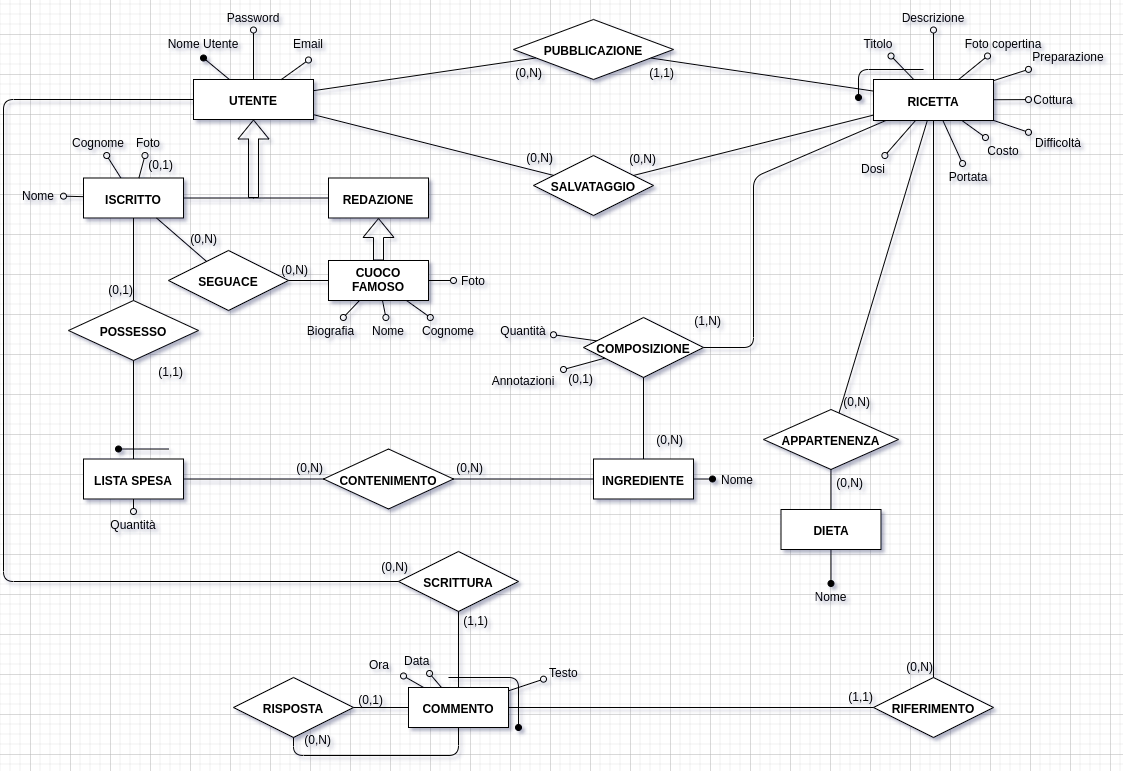
\includegraphics[width=\textwidth]{er1.png}

\subsubsection{Business Rules}
\begin{enumerate}
    % \item Un cuoco famoso non può commentare.
    \item La redazione può solo rispondere ad altri commenti, non può scriverne di autonomi.
    \item La redazione pubblica ricette che possono avere avere come autore un cuoco famoso.
    \item Ad ogni ricetta sono associate delle ricette simili. Due ricette si considerano simili se hanno almeno una categoria in comune e hanno come autore lo stesso cuoco o utente.
    \item Quando un utente cancella la propria iscrizione al sito vengono eliminati: i suoi dati personali, la lista delle ricette preferite, gli ingredienti contenuti nella "lista della spesa" e la lista dei cuochi eventualmente seguiti; mentre vengono mantenute le ricette e i commenti pubblica.
\end{enumerate}


\section{Progettazione logica}
\subsection{Tavola dei volumi}

\vspace{2cm}
    \begin{tabularx}{\textwidth}{X|X|X|X}
    \bfseries CONCETTO     & \bfseries TIPO  & \bfseries VOLUME \\ 
    \hline\hline
    \bfseries Utente        & Entità        & 700.000       \\ 
    \hline
    \bfseries Redazione     & Entità        & 1             \\
    \hline
    \bfseries Iscritto      & Entità        & 699.499       \\
    \hline
    \bfseries Cuoco famoso  & Entità        & 500           \\
    \hline
    \bfseries Ricetta       & Entità        & 10.000        \\
    \hline
    \bfseries Commento      & Entità        & 3.000.000    $300 commenti per ricetta$\\
    \hline
    \bfseries Ingrediente   & Entità        & 1.000         \\
    \hline
    \bfseries Lista Spesa   & Entità        & 699.499       \\
    \hline
    \bfseries Portata       & Entità        & 7             \\
    \hline
    \bfseries Dieta         & Entità        & 6             \\
    \hline
    \bfseries Pubblicazione & Associazione  & 10.000        \\
    \hline
    \bfseries Salvataggio   & Associazione  & 7.000.000     \\
    \hline
    \bfseries Scrittura     & Associazione  & 3.000.000     \\
    \hline
    \bfseries Seguace       & Associazione  & 1.000.000     $56$\\
    \hline
    \bfseries Possesso      & Associazione  & 699.499       $56$\\
    \hline
    \bfseries Risposta      & Associazione  & 5.000.000     $56$\\
    \hline
    \bfseries Riferimento   & Associazione  & 10.000        $56$\\
    \hline
    \bfseries Composizione  & Associazione  & 30.000        $56$\\
    \hline
    \bfseries Contenimento  & Associazione  & 5.000.000     $56$\\
    \hline
    \bfseries Tipologia     & Associazione  & 7             $56$\\
    \hline
    \bfseries Appartenenza  & Associazione  & 6             $56$\\
    \hline
    \end{tabularx}

\begin{itemize}
    \item Gran parte degli utenti utilizzerà il sito per consultare le ricette, una piccola parte di loro le pubblicherà.
    \item Un alto numero di utenti salverà le ricette per poterle consultare in futuro
    \item Gli ingredienti presenti nelle ricette
    \item Ipotizziamo circa $300$ commenti per ricetta
    \item Ipotizziamo un salvataggio di circa 10 ricette per ogni utente
\end{itemize}

\newpage

\subsection{Tavola delle operazioni}

\subsection{Ristrutturazione Schema E-R}
\subsubsection{Analisi delle ridondanze}
\subsubsection{Eliminazione delle generalizzazioni}
\subsubsection{Scelta degli identificatori principali}

\subsection{Schema E-R ristrutturato e Business Rules}

\subsection{Schema Relazionale}

\section{Implementazione}
\subsection{DDL di creazione del Database}

\subsection{DML di popolamento del Database}

\subsection{Operazioni di Cancellazione e Modifica per la verifica dei vincoli e degli effetti causati da operazioni su chiavi esterne}


\end{document}